\documentclass[1p]{elsarticle_modified}
%\bibliographystyle{elsarticle-num}

%\usepackage[colorlinks]{hyperref}
%\usepackage{abbrmath_seonhwa} %\Abb, \Ascr, \Acal ,\Abf, \Afrak
\usepackage{amsfonts}
\usepackage{amssymb}
\usepackage{amsmath}
\usepackage{amsthm}
\usepackage{scalefnt}
\usepackage{amsbsy}
\usepackage{kotex}
\usepackage{caption}
\usepackage{subfig}
\usepackage{color}
\usepackage{graphicx}
\usepackage{xcolor} %% white, black, red, green, blue, cyan, magenta, yellow
\usepackage{float}
\usepackage{setspace}
\usepackage{hyperref}

\usepackage{tikz}
\usetikzlibrary{arrows}

\usepackage{multirow}
\usepackage{array} % fixed length table
\usepackage{hhline}

%%%%%%%%%%%%%%%%%%%%%
\makeatletter
\renewcommand*\env@matrix[1][\arraystretch]{%
	\edef\arraystretch{#1}%
	\hskip -\arraycolsep
	\let\@ifnextchar\new@ifnextchar
	\array{*\c@MaxMatrixCols c}}
\makeatother %https://tex.stackexchange.com/questions/14071/how-can-i-increase-the-line-spacing-in-a-matrix
%%%%%%%%%%%%%%%

\usepackage[normalem]{ulem}

\newcommand{\msout}[1]{\ifmmode\text{\sout{\ensuremath{#1}}}\else\sout{#1}\fi}
%SOURCE: \msout is \stkout macro in https://tex.stackexchange.com/questions/20609/strikeout-in-math-mode

\newcommand{\cancel}[1]{
	\ifmmode
	{\color{red}\msout{#1}}
	\else
	{\color{red}\sout{#1}}
	\fi
}

\newcommand{\add}[1]{
	{\color{blue}\uwave{#1}}
}

\newcommand{\replace}[2]{
	\ifmmode
	{\color{red}\msout{#1}}{\color{blue}\uwave{#2}}
	\else
	{\color{red}\sout{#1}}{\color{blue}\uwave{#2}}
	\fi
}

\newcommand{\Sol}{\mathcal{S}} %segment
\newcommand{\D}{D} %diagram
\newcommand{\A}{\mathcal{A}} %arc


%%%%%%%%%%%%%%%%%%%%%%%%%%%%%5 test

\def\sl{\operatorname{\textup{SL}}(2,\Cbb)}
\def\psl{\operatorname{\textup{PSL}}(2,\Cbb)}
\def\quan{\mkern 1mu \triangleright \mkern 1mu}

\theoremstyle{definition}
\newtheorem{thm}{Theorem}[section]
\newtheorem{prop}[thm]{Proposition}
\newtheorem{lem}[thm]{Lemma}
\newtheorem{ques}[thm]{Question}
\newtheorem{cor}[thm]{Corollary}
\newtheorem{defn}[thm]{Definition}
\newtheorem{exam}[thm]{Example}
\newtheorem{rmk}[thm]{Remark}
\newtheorem{alg}[thm]{Algorithm}

\newcommand{\I}{\sqrt{-1}}
\begin{document}

%\begin{frontmatter}
%
%\title{Boundary parabolic representations of knots up to 8 crossings}
%
%%% Group authors per affiliation:
%\author{Yunhi Cho} 
%\address{Department of Mathematics, University of Seoul, Seoul, Korea}
%\ead{yhcho@uos.ac.kr}
%
%
%\author{Seonhwa Kim} %\fnref{s_kim}}
%\address{Center for Geometry and Physics, Institute for Basic Science, Pohang, 37673, Korea}
%\ead{ryeona17@ibs.re.kr}
%
%\author{Hyuk Kim}
%\address{Department of Mathematical Sciences, Seoul National University, Seoul 08826, Korea}
%\ead{hyukkim@snu.ac.kr}
%
%\author{Seokbeom Yoon}
%\address{Department of Mathematical Sciences, Seoul National University, Seoul, 08826,  Korea}
%\ead{sbyoon15@snu.ac.kr}
%
%\begin{abstract}
%We find all boundary parabolic representation of knots up to 8 crossings.
%
%\end{abstract}
%\begin{keyword}
%    \MSC[2010] 57M25 
%\end{keyword}
%
%\end{frontmatter}

%\linenumbers
%\tableofcontents
%
\newcommand\colored[1]{\textcolor{white}{\rule[-0.35ex]{0.8em}{1.4ex}}\kern-0.8em\color{red} #1}%
%\newcommand\colored[1]{\textcolor{white}{ #1}\kern-2.17ex	\textcolor{white}{ #1}\kern-1.81ex	\textcolor{white}{ #1}\kern-2.15ex\color{red}#1	}

{\Large $\underline{12n_{0272}~(K12n_{0272})}$}

\setlength{\tabcolsep}{10pt}
\renewcommand{\arraystretch}{1.6}
\vspace{1cm}\begin{tabular}{m{100pt}>{\centering\arraybackslash}m{274pt}}
\multirow{5}{120pt}{
	\centering
	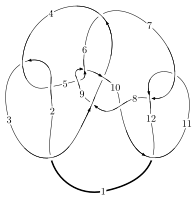
\includegraphics[width=112pt]{../../../GIT/diagram.site/Diagrams/png/2361_12n_0272.png}\\
\ \ \ A knot diagram\footnotemark}&
\allowdisplaybreaks
\textbf{Linearized knot diagam} \\
\cline{2-2}
 &
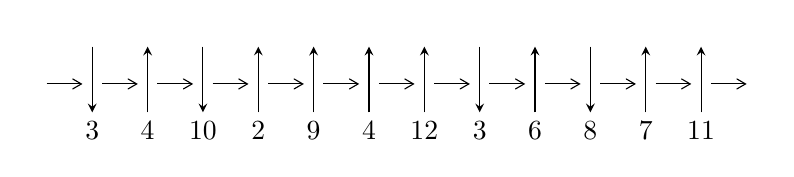
\begin{tikzpicture}[x=20pt, y=17pt]
	% nodes
	\node (C0) at (0, 0) {};
	\node (C1) at (1, 0) {};
	\node (C1U) at (1, +1) {};
	\node (C1D) at (1, -1) {3};

	\node (C2) at (2, 0) {};
	\node (C2U) at (2, +1) {};
	\node (C2D) at (2, -1) {4};

	\node (C3) at (3, 0) {};
	\node (C3U) at (3, +1) {};
	\node (C3D) at (3, -1) {10};

	\node (C4) at (4, 0) {};
	\node (C4U) at (4, +1) {};
	\node (C4D) at (4, -1) {2};

	\node (C5) at (5, 0) {};
	\node (C5U) at (5, +1) {};
	\node (C5D) at (5, -1) {9};

	\node (C6) at (6, 0) {};
	\node (C6U) at (6, +1) {};
	\node (C6D) at (6, -1) {4};

	\node (C7) at (7, 0) {};
	\node (C7U) at (7, +1) {};
	\node (C7D) at (7, -1) {12};

	\node (C8) at (8, 0) {};
	\node (C8U) at (8, +1) {};
	\node (C8D) at (8, -1) {3};

	\node (C9) at (9, 0) {};
	\node (C9U) at (9, +1) {};
	\node (C9D) at (9, -1) {6};

	\node (C10) at (10, 0) {};
	\node (C10U) at (10, +1) {};
	\node (C10D) at (10, -1) {8};

	\node (C11) at (11, 0) {};
	\node (C11U) at (11, +1) {};
	\node (C11D) at (11, -1) {7};

	\node (C12) at (12, 0) {};
	\node (C12U) at (12, +1) {};
	\node (C12D) at (12, -1) {11};
	\node (C13) at (13, 0) {};

	% arrows
	\draw[->,>={angle 60}]
	(C0) edge (C1) (C1) edge (C2) (C2) edge (C3) (C3) edge (C4) (C4) edge (C5) (C5) edge (C6) (C6) edge (C7) (C7) edge (C8) (C8) edge (C9) (C9) edge (C10) (C10) edge (C11) (C11) edge (C12) (C12) edge (C13) ;	\draw[->,>=stealth]
	(C1U) edge (C1D) (C2D) edge (C2U) (C3U) edge (C3D) (C4D) edge (C4U) (C5D) edge (C5U) (C6D) edge (C6U) (C7D) edge (C7U) (C8U) edge (C8D) (C9D) edge (C9U) (C10U) edge (C10D) (C11D) edge (C11U) (C12D) edge (C12U) ;
	\end{tikzpicture} \\
\hhline{~~} \\& 
\textbf{Solving Sequence} \\ \cline{2-2} 
 &
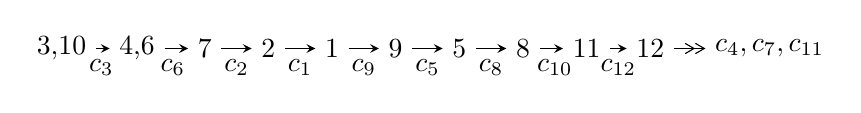
\begin{tikzpicture}[x=23pt, y=7pt]
	% node
	\node (A0) at (-1/8, 0) {3,10};
	\node (A1) at (17/16, 0) {4,6};
	\node (A2) at (17/8, 0) {7};
	\node (A3) at (25/8, 0) {2};
	\node (A4) at (33/8, 0) {1};
	\node (A5) at (41/8, 0) {9};
	\node (A6) at (49/8, 0) {5};
	\node (A7) at (57/8, 0) {8};
	\node (A8) at (65/8, 0) {11};
	\node (A9) at (73/8, 0) {12};
	\node (C1) at (1/2, -1) {$c_{3}$};
	\node (C2) at (13/8, -1) {$c_{6}$};
	\node (C3) at (21/8, -1) {$c_{2}$};
	\node (C4) at (29/8, -1) {$c_{1}$};
	\node (C5) at (37/8, -1) {$c_{9}$};
	\node (C6) at (45/8, -1) {$c_{5}$};
	\node (C7) at (53/8, -1) {$c_{8}$};
	\node (C8) at (61/8, -1) {$c_{10}$};
	\node (C9) at (69/8, -1) {$c_{12}$};
	\node (A10) at (11, 0) {$c_{4},c_{7},c_{11}$};

	% edge
	\draw[->,>=stealth]	
	(A0) edge (A1) (A1) edge (A2) (A2) edge (A3) (A3) edge (A4) (A4) edge (A5) (A5) edge (A6) (A6) edge (A7) (A7) edge (A8) (A8) edge (A9) ;
	\draw[->>,>={angle 60}]	
	(A9) edge (A10);
\end{tikzpicture} \\ 

\end{tabular} \\

\footnotetext{
The image of knot diagram is generated by the software ``\textbf{Draw programme}" developed by Andrew Bartholomew(\url{http://www.layer8.co.uk/maths/draw/index.htm\#Running-draw}), where we modified some parts for our purpose(\url{https://github.com/CATsTAILs/LinksPainter}).
}\phantom \\ \newline 
\centering \textbf{Ideals for irreducible components\footnotemark of $X_{\text{par}}$} 
 
\begin{align*}
I^u_{1}&=\langle 
6.07284\times10^{41} u^{54}+1.52970\times10^{42} u^{53}+\cdots+1.46698\times10^{41} b-3.05374\times10^{42},\\
\phantom{I^u_{1}}&\phantom{= \langle  }-2.49859\times10^{42} u^{54}-5.62187\times10^{42} u^{53}+\cdots+3.66745\times10^{41} a+2.92087\times10^{42},\\
\phantom{I^u_{1}}&\phantom{= \langle  }u^{55}+2 u^{54}+\cdots+16 u-5\rangle \\
I^u_{2}&=\langle 
b^4-8 b^3 u+4 b^3-2 b^2 u-18 b^2+28 b u-20 b+8 u+7,\;a+u-1,\;u^2- u+1\rangle \\
I^u_{3}&=\langle 
b^3+6 b^2 u+3 b^2-9 b-6 u-3,\;a- u-1,\;u^2+u+1\rangle \\
\\
\end{align*}
\raggedright * 3 irreducible components of $\dim_{\mathbb{C}}=0$, with total 69 representations.\\
\footnotetext{All coefficients of polynomials are rational numbers. But the coefficients are sometimes approximated in decimal forms when there is not enough margin.}
\newpage
\renewcommand{\arraystretch}{1}
\centering \section*{I. $I^u_{1}= \langle 6.07\times10^{41} u^{54}+1.53\times10^{42} u^{53}+\cdots+1.47\times10^{41} b-3.05\times10^{42},\;-2.50\times10^{42} u^{54}-5.62\times10^{42} u^{53}+\cdots+3.67\times10^{41} a+2.92\times10^{42},\;u^{55}+2 u^{54}+\cdots+16 u-5 \rangle$}
\flushleft \textbf{(i) Arc colorings}\\
\begin{tabular}{m{7pt} m{180pt} m{7pt} m{180pt} }
\flushright $a_{3}=$&$\begin{pmatrix}1\\0\end{pmatrix}$ \\
\flushright $a_{10}=$&$\begin{pmatrix}0\\u\end{pmatrix}$ \\
\flushright $a_{4}=$&$\begin{pmatrix}1\\u^2\end{pmatrix}$ \\
\flushright $a_{6}=$&$\begin{pmatrix}6.81288 u^{54}+15.3291 u^{53}+\cdots-80.3573 u-7.96431\\-4.13969 u^{54}-10.4275 u^{53}+\cdots+5.97193 u+20.8165\end{pmatrix}$ \\
\flushright $a_{7}=$&$\begin{pmatrix}4.56016 u^{54}+9.52527 u^{53}+\cdots-81.1963 u+4.33551\\-3.61239 u^{54}-8.85323 u^{53}+\cdots+15.4827 u+14.3245\end{pmatrix}$ \\
\flushright $a_{2}=$&$\begin{pmatrix}u^2+1\\u^4\end{pmatrix}$ \\
\flushright $a_{1}=$&$\begin{pmatrix}u^4+u^2+1\\u^4\end{pmatrix}$ \\
\flushright $a_{9}=$&$\begin{pmatrix}0.831512 u^{54}+0.329358 u^{53}+\cdots-66.1006 u+20.4585\\1.43416 u^{54}+0.946480 u^{53}+\cdots-115.254 u+34.1944\end{pmatrix}$ \\
\flushright $a_{5}=$&$\begin{pmatrix}u^4+u^2+1\\u^6+u^2\end{pmatrix}$ \\
\flushright $a_{8}=$&$\begin{pmatrix}2.26567 u^{54}+1.27584 u^{53}+\cdots-181.354 u+54.6529\\1.43416 u^{54}+0.946480 u^{53}+\cdots-115.254 u+34.1944\end{pmatrix}$ \\
\flushright $a_{11}=$&$\begin{pmatrix}-0.582714 u^{54}-5.23624 u^{53}+\cdots-155.359 u+60.0525\\-3.07932 u^{54}-5.89630 u^{53}+\cdots+75.6665 u-11.5791\end{pmatrix}$ \\
\flushright $a_{12}=$&$\begin{pmatrix}3.31418 u^{54}+2.60263 u^{53}+\cdots-230.938 u+66.8664\\-4.10335 u^{54}-10.8910 u^{53}+\cdots-23.6437 u+30.3804\end{pmatrix}$\\&\end{tabular}
\flushleft \textbf{(ii) Obstruction class $= -1$}\\~\\
\flushleft \textbf{(iii) Cusp Shapes $= 2.38419 u^{54}+9.98480 u^{53}+\cdots+165.359 u-64.6148$}\\~\\
\newpage\renewcommand{\arraystretch}{1}
\flushleft \textbf{(iv) u-Polynomials at the component}\newline \\
\begin{tabular}{m{50pt}|m{274pt}}
Crossings & \hspace{64pt}u-Polynomials at each crossing \\
\hline $$\begin{aligned}c_{1}\end{aligned}$$&$\begin{aligned}
&u^{55}+62 u^{54}+\cdots+72966 u-625
\end{aligned}$\\
\hline $$\begin{aligned}c_{2},c_{4}\end{aligned}$$&$\begin{aligned}
&u^{55}-14 u^{54}+\cdots-254 u+25
\end{aligned}$\\
\hline $$\begin{aligned}c_{3}\end{aligned}$$&$\begin{aligned}
&u^{55}+2 u^{54}+\cdots+16 u-5
\end{aligned}$\\
\hline $$\begin{aligned}c_{5},c_{9}\end{aligned}$$&$\begin{aligned}
&u^{55}-3 u^{54}+\cdots-9 u-1
\end{aligned}$\\
\hline $$\begin{aligned}c_{6}\end{aligned}$$&$\begin{aligned}
&u^{55}+6 u^{54}+\cdots+856224 u-220279
\end{aligned}$\\
\hline $$\begin{aligned}c_{7},c_{11}\end{aligned}$$&$\begin{aligned}
&u^{55}- u^{54}+\cdots+12 u-4
\end{aligned}$\\
\hline $$\begin{aligned}c_{8}\end{aligned}$$&$\begin{aligned}
&u^{55}-25 u^{53}+\cdots+116957786 u-39721487
\end{aligned}$\\
\hline $$\begin{aligned}c_{10}\end{aligned}$$&$\begin{aligned}
&u^{55}-3 u^{54}+\cdots+3164 u-748
\end{aligned}$\\
\hline $$\begin{aligned}c_{12}\end{aligned}$$&$\begin{aligned}
&u^{55}-25 u^{54}+\cdots+80 u-16
\end{aligned}$\\
\hline
\end{tabular}\\~\\
\newpage\renewcommand{\arraystretch}{1}
\flushleft \textbf{(v) Riley Polynomials at the component}\newline \\
\begin{tabular}{m{50pt}|m{274pt}}
Crossings & \hspace{64pt}Riley Polynomials at each crossing \\
\hline $$\begin{aligned}c_{1}\end{aligned}$$&$\begin{aligned}
&y^{55}-130 y^{54}+\cdots+3614843406 y-390625
\end{aligned}$\\
\hline $$\begin{aligned}c_{2},c_{4}\end{aligned}$$&$\begin{aligned}
&y^{55}+62 y^{54}+\cdots+72966 y-625
\end{aligned}$\\
\hline $$\begin{aligned}c_{3}\end{aligned}$$&$\begin{aligned}
&y^{55}+14 y^{54}+\cdots-254 y-25
\end{aligned}$\\
\hline $$\begin{aligned}c_{5},c_{9}\end{aligned}$$&$\begin{aligned}
&y^{55}-15 y^{54}+\cdots+43 y-1
\end{aligned}$\\
\hline $$\begin{aligned}c_{6}\end{aligned}$$&$\begin{aligned}
&y^{55}+46 y^{54}+\cdots-1179952912654 y-48522837841
\end{aligned}$\\
\hline $$\begin{aligned}c_{7},c_{11}\end{aligned}$$&$\begin{aligned}
&y^{55}-25 y^{54}+\cdots+80 y-16
\end{aligned}$\\
\hline $$\begin{aligned}c_{8}\end{aligned}$$&$\begin{aligned}
&y^{55}-50 y^{54}+\cdots+12865645844702842 y-1577796529491169
\end{aligned}$\\
\hline $$\begin{aligned}c_{10}\end{aligned}$$&$\begin{aligned}
&y^{55}-5 y^{54}+\cdots+5379280 y-559504
\end{aligned}$\\
\hline $$\begin{aligned}c_{12}\end{aligned}$$&$\begin{aligned}
&y^{55}+15 y^{54}+\cdots-2816 y-256
\end{aligned}$\\
\hline
\end{tabular}\\~\\
\newpage\flushleft \textbf{(vi) Complex Volumes and Cusp Shapes}
$$\begin{array}{c|c|c}  
\text{Solutions to }I^u_{1}& \I (\text{vol} + \sqrt{-1}CS) & \text{Cusp shape}\\
 \hline 
\begin{aligned}
u &= \phantom{-}0.643133 + 0.772247 I \\
a &= \phantom{-}0.073099 + 0.590591 I \\
b &= \phantom{-}0.874696 - 0.160448 I\end{aligned}
 & \phantom{-}2.22767 - 6.23387 I & \phantom{-}3.64860 + 7.74824 I \\ \hline\begin{aligned}
u &= \phantom{-}0.643133 - 0.772247 I \\
a &= \phantom{-}0.073099 - 0.590591 I \\
b &= \phantom{-}0.874696 + 0.160448 I\end{aligned}
 & \phantom{-}2.22767 + 6.23387 I & \phantom{-}3.64860 - 7.74824 I \\ \hline\begin{aligned}
u &= \phantom{-}0.541644 + 0.828095 I \\
a &= -0.038556 + 0.200004 I \\
b &= \phantom{-}0.699024 + 0.702967 I\end{aligned}
 & \phantom{-}2.49097 + 1.59610 I & \phantom{-}3.71601 - 0.32055 I \\ \hline\begin{aligned}
u &= \phantom{-}0.541644 - 0.828095 I \\
a &= -0.038556 - 0.200004 I \\
b &= \phantom{-}0.699024 - 0.702967 I\end{aligned}
 & \phantom{-}2.49097 - 1.59610 I & \phantom{-}3.71601 + 0.32055 I \\ \hline\begin{aligned}
u &= \phantom{-}0.255352 + 0.947684 I \\
a &= \phantom{-}0.566764 - 0.140113 I \\
b &= -0.528106 + 0.715239 I\end{aligned}
 & \phantom{-}2.15852 + 1.39769 I & \phantom{-}6.44233 - 2.55277 I \\ \hline\begin{aligned}
u &= \phantom{-}0.255352 - 0.947684 I \\
a &= \phantom{-}0.566764 + 0.140113 I \\
b &= -0.528106 - 0.715239 I\end{aligned}
 & \phantom{-}2.15852 - 1.39769 I & \phantom{-}6.44233 + 2.55277 I \\ \hline\begin{aligned}
u &= -0.733192 + 0.713911 I \\
a &= \phantom{-}0.798061 + 1.026100 I \\
b &= \phantom{-}0.52397 - 1.64587 I\end{aligned}
 & \phantom{-}1.34086 + 4.85814 I & \phantom{-}3.75921 - 6.24399 I \\ \hline\begin{aligned}
u &= -0.733192 - 0.713911 I \\
a &= \phantom{-}0.798061 - 1.026100 I \\
b &= \phantom{-}0.52397 + 1.64587 I\end{aligned}
 & \phantom{-}1.34086 - 4.85814 I & \phantom{-}3.75921 + 6.24399 I \\ \hline\begin{aligned}
u &= \phantom{-}0.245931 + 1.003490 I \\
a &= -0.180150 - 0.972673 I \\
b &= \phantom{-}0.19661 + 2.31761 I\end{aligned}
 & \phantom{-}3.99628 - 2.15960 I & \phantom{-}12.20326 + 3.54467 I \\ \hline\begin{aligned}
u &= \phantom{-}0.245931 - 1.003490 I \\
a &= -0.180150 + 0.972673 I \\
b &= \phantom{-}0.19661 - 2.31761 I\end{aligned}
 & \phantom{-}3.99628 + 2.15960 I & \phantom{-}12.20326 - 3.54467 I\\
 \hline 
 \end{array}$$\newpage$$\begin{array}{c|c|c}  
\text{Solutions to }I^u_{1}& \I (\text{vol} + \sqrt{-1}CS) & \text{Cusp shape}\\
 \hline 
\begin{aligned}
u &= -0.455933 + 0.952453 I \\
a &= -0.015920 + 0.377752 I \\
b &= \phantom{-}0.410151 - 1.298800 I\end{aligned}
 & \phantom{-}0.26235 + 2.25660 I & \phantom{-0.000000 } 0. - 4.04903 I \\ \hline\begin{aligned}
u &= -0.455933 - 0.952453 I \\
a &= -0.015920 - 0.377752 I \\
b &= \phantom{-}0.410151 + 1.298800 I\end{aligned}
 & \phantom{-}0.26235 - 2.25660 I & \phantom{-0.000000 -}0. + 4.04903 I \\ \hline\begin{aligned}
u &= -0.613118 + 0.670633 I \\
a &= \phantom{-}0.285325 - 0.526308 I \\
b &= \phantom{-}0.430171 - 0.004191 I\end{aligned}
 & -0.67943 + 1.91424 I & -0.34235 - 3.72747 I \\ \hline\begin{aligned}
u &= -0.613118 - 0.670633 I \\
a &= \phantom{-}0.285325 + 0.526308 I \\
b &= \phantom{-}0.430171 + 0.004191 I\end{aligned}
 & -0.67943 - 1.91424 I & -0.34235 + 3.72747 I \\ \hline\begin{aligned}
u &= -0.629710 + 0.956216 I \\
a &= \phantom{-}0.732740 + 0.781573 I \\
b &= \phantom{-}0.00414 - 2.05580 I\end{aligned}
 & \phantom{-}2.14605 + 0.34842 I & \phantom{-0.000000 } 0 \\ \hline\begin{aligned}
u &= -0.629710 - 0.956216 I \\
a &= \phantom{-}0.732740 - 0.781573 I \\
b &= \phantom{-}0.00414 + 2.05580 I\end{aligned}
 & \phantom{-}2.14605 - 0.34842 I & \phantom{-0.000000 } 0 \\ \hline\begin{aligned}
u &= -0.778599 + 0.329602 I \\
a &= \phantom{-}0.678856 - 0.803797 I \\
b &= \phantom{-}0.168770 - 0.052346 I\end{aligned}
 & -2.66054 + 0.76259 I & -1.67387 - 1.84877 I \\ \hline\begin{aligned}
u &= -0.778599 - 0.329602 I \\
a &= \phantom{-}0.678856 + 0.803797 I \\
b &= \phantom{-}0.168770 + 0.052346 I\end{aligned}
 & -2.66054 - 0.76259 I & -1.67387 + 1.84877 I \\ \hline\begin{aligned}
u &= \phantom{-}0.516920 + 1.032630 I \\
a &= \phantom{-}0.675627 - 0.596738 I \\
b &= -0.38124 + 1.87533 I\end{aligned}
 & \phantom{-}2.33972 - 3.94259 I & \phantom{-0.000000 } 0 \\ \hline\begin{aligned}
u &= \phantom{-}0.516920 - 1.032630 I \\
a &= \phantom{-}0.675627 + 0.596738 I \\
b &= -0.38124 - 1.87533 I\end{aligned}
 & \phantom{-}2.33972 + 3.94259 I & \phantom{-0.000000 } 0\\
 \hline 
 \end{array}$$\newpage$$\begin{array}{c|c|c}  
\text{Solutions to }I^u_{1}& \I (\text{vol} + \sqrt{-1}CS) & \text{Cusp shape}\\
 \hline 
\begin{aligned}
u &= \phantom{-}0.826976 + 0.174508 I \\
a &= \phantom{-}0.793904 + 0.895765 I \\
b &= \phantom{-}0.301796 + 0.056023 I\end{aligned}
 & -1.77909 + 4.14857 I & \phantom{-}0.53786 - 4.76792 I \\ \hline\begin{aligned}
u &= \phantom{-}0.826976 - 0.174508 I \\
a &= \phantom{-}0.793904 - 0.895765 I \\
b &= \phantom{-}0.301796 - 0.056023 I\end{aligned}
 & -1.77909 - 4.14857 I & \phantom{-}0.53786 + 4.76792 I \\ \hline\begin{aligned}
u &= -0.403926 + 1.086140 I \\
a &= -0.301206 + 0.696568 I \\
b &= \phantom{-}0.84782 - 1.88492 I\end{aligned}
 & -0.05616 + 3.61985 I & \phantom{-0.000000 } 0 \\ \hline\begin{aligned}
u &= -0.403926 - 1.086140 I \\
a &= -0.301206 - 0.696568 I \\
b &= \phantom{-}0.84782 + 1.88492 I\end{aligned}
 & -0.05616 - 3.61985 I & \phantom{-0.000000 } 0 \\ \hline\begin{aligned}
u &= \phantom{-}0.635290 + 0.539955 I \\
a &= \phantom{-}0.80977 - 1.17532 I \\
b &= \phantom{-}0.335753 + 1.218400 I\end{aligned}
 & \phantom{-}0.699297 - 0.586817 I & \phantom{-}2.30186 - 0.73142 I \\ \hline\begin{aligned}
u &= \phantom{-}0.635290 - 0.539955 I \\
a &= \phantom{-}0.80977 + 1.17532 I \\
b &= \phantom{-}0.335753 - 1.218400 I\end{aligned}
 & \phantom{-}0.699297 + 0.586817 I & \phantom{-}2.30186 + 0.73142 I \\ \hline\begin{aligned}
u &= \phantom{-}0.357804 + 1.146380 I \\
a &= -0.371516 - 0.795743 I \\
b &= \phantom{-}0.99860 + 2.21220 I\end{aligned}
 & \phantom{-}1.55711 - 8.45299 I & \phantom{-0.000000 } 0 \\ \hline\begin{aligned}
u &= \phantom{-}0.357804 - 1.146380 I \\
a &= -0.371516 + 0.795743 I \\
b &= \phantom{-}0.99860 - 2.21220 I\end{aligned}
 & \phantom{-}1.55711 + 8.45299 I & \phantom{-0.000000 } 0 \\ \hline\begin{aligned}
u &= -0.889584 + 0.849382 I \\
a &= -1.053920 + 0.046965 I \\
b &= \phantom{-}0.026656 + 0.258349 I\end{aligned}
 & -3.64967 - 0.17207 I & \phantom{-0.000000 } 0 \\ \hline\begin{aligned}
u &= -0.889584 - 0.849382 I \\
a &= -1.053920 - 0.046965 I \\
b &= \phantom{-}0.026656 - 0.258349 I\end{aligned}
 & -3.64967 + 0.17207 I & \phantom{-0.000000 } 0\\
 \hline 
 \end{array}$$\newpage$$\begin{array}{c|c|c}  
\text{Solutions to }I^u_{1}& \I (\text{vol} + \sqrt{-1}CS) & \text{Cusp shape}\\
 \hline 
\begin{aligned}
u &= -0.031113 + 0.765896 I \\
a &= -0.25903 + 1.40965 I \\
b &= -1.01707 - 2.10431 I\end{aligned}
 & \phantom{-}5.48181 + 3.63285 I & \phantom{-}13.5953 - 4.3642 I \\ \hline\begin{aligned}
u &= -0.031113 - 0.765896 I \\
a &= -0.25903 - 1.40965 I \\
b &= -1.01707 + 2.10431 I\end{aligned}
 & \phantom{-}5.48181 - 3.63285 I & \phantom{-}13.5953 + 4.3642 I \\ \hline\begin{aligned}
u &= -0.980350 + 0.786429 I \\
a &= -1.188620 + 0.046193 I \\
b &= -0.330725 + 0.677000 I\end{aligned}
 & -7.75967 - 8.08659 I & \phantom{-0.000000 } 0 \\ \hline\begin{aligned}
u &= -0.980350 - 0.786429 I \\
a &= -1.188620 - 0.046193 I \\
b &= -0.330725 - 0.677000 I\end{aligned}
 & -7.75967 + 8.08659 I & \phantom{-0.000000 } 0 \\ \hline\begin{aligned}
u &= \phantom{-}0.973285 + 0.826962 I \\
a &= -1.156140 - 0.078168 I \\
b &= -0.129976 - 0.669159 I\end{aligned}
 & -9.70239 + 2.43605 I & \phantom{-0.000000 } 0 \\ \hline\begin{aligned}
u &= \phantom{-}0.973285 - 0.826962 I \\
a &= -1.156140 + 0.078168 I \\
b &= -0.129976 + 0.669159 I\end{aligned}
 & -9.70239 - 2.43605 I & \phantom{-0.000000 } 0 \\ \hline\begin{aligned}
u &= -0.834739 + 0.982712 I \\
a &= \phantom{-}0.003646 - 1.048060 I \\
b &= -0.34032 + 2.13272 I\end{aligned}
 & -3.22528 + 6.57102 I & \phantom{-0.000000 } 0 \\ \hline\begin{aligned}
u &= -0.834739 - 0.982712 I \\
a &= \phantom{-}0.003646 + 1.048060 I \\
b &= -0.34032 - 2.13272 I\end{aligned}
 & -3.22528 - 6.57102 I & \phantom{-0.000000 } 0 \\ \hline\begin{aligned}
u &= -0.941255 + 0.925932 I \\
a &= \phantom{-}0.118357 - 1.083720 I \\
b &= -0.82877 + 1.42918 I\end{aligned}
 & -8.54383 - 0.44596 I & \phantom{-0.000000 } 0 \\ \hline\begin{aligned}
u &= -0.941255 - 0.925932 I \\
a &= \phantom{-}0.118357 + 1.083720 I \\
b &= -0.82877 - 1.42918 I\end{aligned}
 & -8.54383 + 0.44596 I & \phantom{-0.000000 } 0\\
 \hline 
 \end{array}$$\newpage$$\begin{array}{c|c|c}  
\text{Solutions to }I^u_{1}& \I (\text{vol} + \sqrt{-1}CS) & \text{Cusp shape}\\
 \hline 
\begin{aligned}
u &= \phantom{-}0.939126 + 0.931067 I \\
a &= -1.066090 - 0.168051 I \\
b &= \phantom{-}0.426943 - 0.559972 I\end{aligned}
 & -10.06640 - 1.58825 I & \phantom{-0.000000 } 0 \\ \hline\begin{aligned}
u &= \phantom{-}0.939126 - 0.931067 I \\
a &= -1.066090 + 0.168051 I \\
b &= \phantom{-}0.426943 + 0.559972 I\end{aligned}
 & -10.06640 + 1.58825 I & \phantom{-0.000000 } 0 \\ \hline\begin{aligned}
u &= -0.917840 + 0.968985 I \\
a &= -1.027200 + 0.203661 I \\
b &= \phantom{-}0.641384 + 0.467628 I\end{aligned}
 & -8.40289 + 7.27332 I & \phantom{-0.000000 } 0 \\ \hline\begin{aligned}
u &= -0.917840 - 0.968985 I \\
a &= -1.027200 - 0.203661 I \\
b &= \phantom{-}0.641384 - 0.467628 I\end{aligned}
 & -8.40289 - 7.27332 I & \phantom{-0.000000 } 0 \\ \hline\begin{aligned}
u &= \phantom{-}0.921796 + 0.966607 I \\
a &= \phantom{-}0.077249 + 1.095330 I \\
b &= -0.84619 - 1.72543 I\end{aligned}
 & -9.95240 - 5.24724 I & \phantom{-0.000000 } 0 \\ \hline\begin{aligned}
u &= \phantom{-}0.921796 - 0.966607 I \\
a &= \phantom{-}0.077249 - 1.095330 I \\
b &= -0.84619 + 1.72543 I\end{aligned}
 & -9.95240 + 5.24724 I & \phantom{-0.000000 } 0 \\ \hline\begin{aligned}
u &= \phantom{-}0.861727 + 1.038620 I \\
a &= -0.009790 + 1.107290 I \\
b &= -0.74617 - 2.39826 I\end{aligned}
 & -9.01329 - 9.17083 I & \phantom{-0.000000 } 0 \\ \hline\begin{aligned}
u &= \phantom{-}0.861727 - 1.038620 I \\
a &= -0.009790 - 1.107290 I \\
b &= -0.74617 + 2.39826 I\end{aligned}
 & -9.01329 + 9.17083 I & \phantom{-0.000000 } 0 \\ \hline\begin{aligned}
u &= -0.840461 + 1.058680 I \\
a &= -0.036507 - 1.110470 I \\
b &= -0.69938 + 2.61952 I\end{aligned}
 & -6.8786 + 14.7636 I & \phantom{-0.000000 } 0 \\ \hline\begin{aligned}
u &= -0.840461 - 1.058680 I \\
a &= -0.036507 + 1.110470 I \\
b &= -0.69938 - 2.61952 I\end{aligned}
 & -6.8786 - 14.7636 I & \phantom{-0.000000 } 0\\
 \hline 
 \end{array}$$\newpage$$\begin{array}{c|c|c}  
\text{Solutions to }I^u_{1}& \I (\text{vol} + \sqrt{-1}CS) & \text{Cusp shape}\\
 \hline 
\begin{aligned}
u &= \phantom{-}0.076743 + 0.576649 I \\
a &= -0.56089 + 1.77985 I \\
b &= -1.50038 - 1.35769 I\end{aligned}
 & \phantom{-}4.70804 - 3.84497 I & \phantom{-}11.03034 + 2.81257 I \\ \hline\begin{aligned}
u &= \phantom{-}0.076743 - 0.576649 I \\
a &= -0.56089 - 1.77985 I \\
b &= -1.50038 + 1.35769 I\end{aligned}
 & \phantom{-}4.70804 + 3.84497 I & \phantom{-}11.03034 - 2.81257 I \\ \hline\begin{aligned}
u &= \phantom{-}0.094139 + 0.557159 I \\
a &= -0.04524 - 1.86661 I \\
b &= -0.91864 + 1.34124 I\end{aligned}
 & \phantom{-}2.17167 - 0.44148 I & \phantom{-}7.35335 + 0.00703 I \\ \hline\begin{aligned}
u &= \phantom{-}0.094139 - 0.557159 I \\
a &= -0.04524 + 1.86661 I \\
b &= -0.91864 - 1.34124 I\end{aligned}
 & \phantom{-}2.17167 + 0.44148 I & \phantom{-}7.35335 - 0.00703 I \\ \hline\begin{aligned}
u &= \phantom{-}0.319907\phantom{ +0.000000I} \\
a &= \phantom{-}2.19474\phantom{ +0.000000I} \\
b &= -0.239033\phantom{ +0.000000I}\end{aligned}
 & \phantom{-}1.23747\phantom{ +0.000000I} & \phantom{-}7.46610\phantom{ +0.000000I}\\
 \hline 
 \end{array}$$\newpage\newpage\renewcommand{\arraystretch}{1}
\centering \section*{II. $I^u_{2}= \langle -8 b^3 u-2 b^2 u+\cdots-20 b+7,\;a+u-1,\;u^2- u+1 \rangle$}
\flushleft \textbf{(i) Arc colorings}\\
\begin{tabular}{m{7pt} m{180pt} m{7pt} m{180pt} }
\flushright $a_{3}=$&$\begin{pmatrix}1\\0\end{pmatrix}$ \\
\flushright $a_{10}=$&$\begin{pmatrix}0\\u\end{pmatrix}$ \\
\flushright $a_{4}=$&$\begin{pmatrix}1\\u-1\end{pmatrix}$ \\
\flushright $a_{6}=$&$\begin{pmatrix}- u+1\\b\end{pmatrix}$ \\
\flushright $a_{7}=$&$\begin{pmatrix}b-2 u+1\\b u+1\end{pmatrix}$ \\
\flushright $a_{2}=$&$\begin{pmatrix}u\\- u\end{pmatrix}$ \\
\flushright $a_{1}=$&$\begin{pmatrix}0\\- u\end{pmatrix}$ \\
\flushright $a_{9}=$&$\begin{pmatrix}u-1\\- b+u\end{pmatrix}$ \\
\flushright $a_{5}=$&$\begin{pmatrix}0\\u\end{pmatrix}$ \\
\flushright $a_{8}=$&$\begin{pmatrix}- b+2 u-1\\- b+u\end{pmatrix}$ \\
\flushright $a_{11}=$&$\begin{pmatrix}- b^2 u+2 b u-4 b+3 u\\- b^2 u+2 b u-3 b+2 u+1\end{pmatrix}$ \\
\flushright $a_{12}=$&$\begin{pmatrix}-2 b^2 u+4 b u-8 b+8 u-2\\- b^3 u+b^3-5 b^2 u-2 b^2+9 b u-15 b+10 u-2\end{pmatrix}$\\&\end{tabular}
\flushleft \textbf{(ii) Obstruction class $= 1$}\\~\\
\flushleft \textbf{(iii) Cusp Shapes $= 4 b^2 u-4 b^2+8 b u+8 b-8 u+24$}\\~\\
\newpage\renewcommand{\arraystretch}{1}
\flushleft \textbf{(iv) u-Polynomials at the component}\newline \\
\begin{tabular}{m{50pt}|m{274pt}}
Crossings & \hspace{64pt}u-Polynomials at each crossing \\
\hline $$\begin{aligned}c_{1},c_{3},c_{4}\end{aligned}$$&$\begin{aligned}
&(u^2- u+1)^4
\end{aligned}$\\
\hline $$\begin{aligned}c_{2}\end{aligned}$$&$\begin{aligned}
&(u^2+u+1)^4
\end{aligned}$\\
\hline $$\begin{aligned}c_{5}\end{aligned}$$&$\begin{aligned}
&(u-1)^8
\end{aligned}$\\
\hline $$\begin{aligned}c_{6}\end{aligned}$$&$\begin{aligned}
&u^8-4 u^7+8 u^6-16 u^5+27 u^4-24 u^3+24 u^2-40 u+25
\end{aligned}$\\
\hline $$\begin{aligned}c_{7},c_{11}\end{aligned}$$&$\begin{aligned}
&(u^4-2 u^2+2)^2
\end{aligned}$\\
\hline $$\begin{aligned}c_{8}\end{aligned}$$&$\begin{aligned}
&u^8+4 u^7+8 u^6+16 u^5+27 u^4+24 u^3+24 u^2+40 u+25
\end{aligned}$\\
\hline $$\begin{aligned}c_{9}\end{aligned}$$&$\begin{aligned}
&(u+1)^8
\end{aligned}$\\
\hline $$\begin{aligned}c_{10}\end{aligned}$$&$\begin{aligned}
&(u^4+2 u^2+2)^2
\end{aligned}$\\
\hline $$\begin{aligned}c_{12}\end{aligned}$$&$\begin{aligned}
&(u^2-2 u+2)^4
\end{aligned}$\\
\hline
\end{tabular}\\~\\
\newpage\renewcommand{\arraystretch}{1}
\flushleft \textbf{(v) Riley Polynomials at the component}\newline \\
\begin{tabular}{m{50pt}|m{274pt}}
Crossings & \hspace{64pt}Riley Polynomials at each crossing \\
\hline $$\begin{aligned}c_{1},c_{2},c_{3}\\c_{4}\end{aligned}$$&$\begin{aligned}
&(y^2+y+1)^4
\end{aligned}$\\
\hline $$\begin{aligned}c_{5},c_{9}\end{aligned}$$&$\begin{aligned}
&(y-1)^8
\end{aligned}$\\
\hline $$\begin{aligned}c_{6},c_{8}\end{aligned}$$&$\begin{aligned}
&y^8-10 y^6+32 y^5+75 y^4-160 y^3+6 y^2-400 y+625
\end{aligned}$\\
\hline $$\begin{aligned}c_{7},c_{11}\end{aligned}$$&$\begin{aligned}
&(y^2-2 y+2)^4
\end{aligned}$\\
\hline $$\begin{aligned}c_{10}\end{aligned}$$&$\begin{aligned}
&(y^2+2 y+2)^4
\end{aligned}$\\
\hline $$\begin{aligned}c_{12}\end{aligned}$$&$\begin{aligned}
&(y^2+4)^4
\end{aligned}$\\
\hline
\end{tabular}\\~\\
\newpage\flushleft \textbf{(vi) Complex Volumes and Cusp Shapes}
$$\begin{array}{c|c|c}  
\text{Solutions to }I^u_{2}& \I (\text{vol} + \sqrt{-1}CS) & \text{Cusp shape}\\
 \hline 
\begin{aligned}
u &= \phantom{-}0.500000 + 0.866025 I \\
a &= \phantom{-}0.500000 - 0.866025 I \\
b &= -0.723943 + 0.788589 I\end{aligned}
 & \phantom{-}4.11234 + 1.63398 I & \phantom{-}10.00000 - 0.53590 I \\ \hline\begin{aligned}
u &= \phantom{-}0.500000 + 0.866025 I \\
a &= \phantom{-}0.500000 - 0.866025 I \\
b &= -1.17903 + 1.57683 I\end{aligned}
 & \phantom{-}4.11234 - 5.69375 I & \phantom{-}10.00000 + 7.46410 I \\ \hline\begin{aligned}
u &= \phantom{-}0.500000 + 0.866025 I \\
a &= \phantom{-}0.500000 - 0.866025 I \\
b &= \phantom{-}1.17903 + 1.88727 I\end{aligned}
 & \phantom{-}4.11234 - 5.69375 I & \phantom{-}10.00000 + 7.46410 I \\ \hline\begin{aligned}
u &= \phantom{-}0.500000 + 0.866025 I \\
a &= \phantom{-}0.500000 - 0.866025 I \\
b &= \phantom{-}0.72394 + 2.67551 I\end{aligned}
 & \phantom{-}4.11234 + 1.63398 I & \phantom{-}10.00000 - 0.53590 I \\ \hline\begin{aligned}
u &= \phantom{-}0.500000 - 0.866025 I \\
a &= \phantom{-}0.500000 + 0.866025 I \\
b &= -0.723943 - 0.788589 I\end{aligned}
 & \phantom{-}4.11234 - 1.63398 I & \phantom{-}10.00000 + 0.53590 I \\ \hline\begin{aligned}
u &= \phantom{-}0.500000 - 0.866025 I \\
a &= \phantom{-}0.500000 + 0.866025 I \\
b &= -1.17903 - 1.57683 I\end{aligned}
 & \phantom{-}4.11234 + 5.69375 I & \phantom{-}10.00000 - 7.46410 I \\ \hline\begin{aligned}
u &= \phantom{-}0.500000 - 0.866025 I \\
a &= \phantom{-}0.500000 + 0.866025 I \\
b &= \phantom{-}1.17903 - 1.88727 I\end{aligned}
 & \phantom{-}4.11234 + 5.69375 I & \phantom{-}10.00000 - 7.46410 I \\ \hline\begin{aligned}
u &= \phantom{-}0.500000 - 0.866025 I \\
a &= \phantom{-}0.500000 + 0.866025 I \\
b &= \phantom{-}0.72394 - 2.67551 I\end{aligned}
 & \phantom{-}4.11234 - 1.63398 I & \phantom{-}10.00000 + 0.53590 I\\
 \hline 
 \end{array}$$\newpage\newpage\renewcommand{\arraystretch}{1}
\centering \section*{III. $I^u_{3}= \langle b^3+6 b^2 u+3 b^2-9 b-6 u-3,\;a- u-1,\;u^2+u+1 \rangle$}
\flushleft \textbf{(i) Arc colorings}\\
\begin{tabular}{m{7pt} m{180pt} m{7pt} m{180pt} }
\flushright $a_{3}=$&$\begin{pmatrix}1\\0\end{pmatrix}$ \\
\flushright $a_{10}=$&$\begin{pmatrix}0\\u\end{pmatrix}$ \\
\flushright $a_{4}=$&$\begin{pmatrix}1\\- u-1\end{pmatrix}$ \\
\flushright $a_{6}=$&$\begin{pmatrix}u+1\\b\end{pmatrix}$ \\
\flushright $a_{7}=$&$\begin{pmatrix}b+2 u+1\\- b u+1\end{pmatrix}$ \\
\flushright $a_{2}=$&$\begin{pmatrix}- u\\u\end{pmatrix}$ \\
\flushright $a_{1}=$&$\begin{pmatrix}0\\u\end{pmatrix}$ \\
\flushright $a_{9}=$&$\begin{pmatrix}u+1\\b+u\end{pmatrix}$ \\
\flushright $a_{5}=$&$\begin{pmatrix}0\\- u\end{pmatrix}$ \\
\flushright $a_{8}=$&$\begin{pmatrix}b+2 u+1\\b+u\end{pmatrix}$ \\
\flushright $a_{11}=$&$\begin{pmatrix}- b^2 u+2 b u+4 b+3 u\\- b^2 u+2 b u+3 b+2 u-1\end{pmatrix}$ \\
\flushright $a_{12}=$&$\begin{pmatrix}0\\b^2+4 b u+2 b+u-3\end{pmatrix}$\\&\end{tabular}
\flushleft \textbf{(ii) Obstruction class $= 1$}\\~\\
\flushleft \textbf{(iii) Cusp Shapes $= -2 b^2 u-2 b^2-4 b u+4 b+2 u+10$}\\~\\
\newpage\renewcommand{\arraystretch}{1}
\flushleft \textbf{(iv) u-Polynomials at the component}\newline \\
\begin{tabular}{m{50pt}|m{274pt}}
Crossings & \hspace{64pt}u-Polynomials at each crossing \\
\hline $$\begin{aligned}c_{1},c_{4},c_{6}\\c_{8}\end{aligned}$$&$\begin{aligned}
&(u^2- u+1)^3
\end{aligned}$\\
\hline $$\begin{aligned}c_{2},c_{3}\end{aligned}$$&$\begin{aligned}
&(u^2+u+1)^3
\end{aligned}$\\
\hline $$\begin{aligned}c_{5}\end{aligned}$$&$\begin{aligned}
&(u+1)^6
\end{aligned}$\\
\hline $$\begin{aligned}c_{7},c_{10},c_{11}\\c_{12}\end{aligned}$$&$\begin{aligned}
&u^6
\end{aligned}$\\
\hline $$\begin{aligned}c_{9}\end{aligned}$$&$\begin{aligned}
&(u-1)^6
\end{aligned}$\\
\hline
\end{tabular}\\~\\
\newpage\renewcommand{\arraystretch}{1}
\flushleft \textbf{(v) Riley Polynomials at the component}\newline \\
\begin{tabular}{m{50pt}|m{274pt}}
Crossings & \hspace{64pt}Riley Polynomials at each crossing \\
\hline $$\begin{aligned}c_{1},c_{2},c_{3}\\c_{4},c_{6},c_{8}\end{aligned}$$&$\begin{aligned}
&(y^2+y+1)^3
\end{aligned}$\\
\hline $$\begin{aligned}c_{5},c_{9}\end{aligned}$$&$\begin{aligned}
&(y-1)^6
\end{aligned}$\\
\hline $$\begin{aligned}c_{7},c_{10},c_{11}\\c_{12}\end{aligned}$$&$\begin{aligned}
&y^6
\end{aligned}$\\
\hline
\end{tabular}\\~\\
\newpage\flushleft \textbf{(vi) Complex Volumes and Cusp Shapes}
$$\begin{array}{c|c|c}  
\text{Solutions to }I^u_{3}& \I (\text{vol} + \sqrt{-1}CS) & \text{Cusp shape}\\
 \hline 
\begin{aligned}
u &= -0.500000 + 0.866025 I \\
a &= \phantom{-}0.500000 + 0.866025 I \\
b &= \phantom{-0.000000 } -1.73205 I\end{aligned}
 & \phantom{-}1.64493 + 2.02988 I & \phantom{-}6.00000 - 3.46410 I \\ \hline\begin{aligned}
u &= -0.500000 + 0.866025 I \\
a &= \phantom{-}0.500000 + 0.866025 I \\
b &= \phantom{-0.000000 } -1.73205 I\end{aligned}
 & \phantom{-}1.64493 + 2.02988 I & \phantom{-}6.00000 - 3.46410 I \\ \hline\begin{aligned}
u &= -0.500000 + 0.866025 I \\
a &= \phantom{-}0.500000 + 0.866025 I \\
b &= \phantom{-0.000000 } -1.73205 I\end{aligned}
 & \phantom{-}1.64493 + 2.02988 I & \phantom{-}6.00000 - 3.46410 I \\ \hline\begin{aligned}
u &= -0.500000 - 0.866025 I \\
a &= \phantom{-}0.500000 - 0.866025 I \\
b &= \phantom{-0.000000 -}1.73205 I\end{aligned}
 & \phantom{-}1.64493 - 2.02988 I & \phantom{-}6.00000 + 3.46410 I \\ \hline\begin{aligned}
u &= -0.500000 - 0.866025 I \\
a &= \phantom{-}0.500000 - 0.866025 I \\
b &= \phantom{-0.000000 -}1.73205 I\end{aligned}
 & \phantom{-}1.64493 - 2.02988 I & \phantom{-}6.00000 + 3.46410 I \\ \hline\begin{aligned}
u &= -0.500000 - 0.866025 I \\
a &= \phantom{-}0.500000 - 0.866025 I \\
b &= \phantom{-0.000000 -}1.73205 I\end{aligned}
 & \phantom{-}1.64493 - 2.02988 I & \phantom{-}6.00000 + 3.46410 I\\
 \hline 
 \end{array}$$\newpage
\newpage\renewcommand{\arraystretch}{1}
\centering \section*{ IV. u-Polynomials}
\begin{tabular}{m{50pt}|m{274pt}}
Crossings & \hspace{64pt}u-Polynomials at each crossing \\
\hline $$\begin{aligned}c_{1}\end{aligned}$$&$\begin{aligned}
&((u^2- u+1)^7)(u^{55}+62 u^{54}+\cdots+72966 u-625)
\end{aligned}$\\
\hline $$\begin{aligned}c_{2}\end{aligned}$$&$\begin{aligned}
&((u^2+u+1)^7)(u^{55}-14 u^{54}+\cdots-254 u+25)
\end{aligned}$\\
\hline $$\begin{aligned}c_{3}\end{aligned}$$&$\begin{aligned}
&((u^2- u+1)^4)(u^2+u+1)^3(u^{55}+2 u^{54}+\cdots+16 u-5)
\end{aligned}$\\
\hline $$\begin{aligned}c_{4}\end{aligned}$$&$\begin{aligned}
&((u^2- u+1)^7)(u^{55}-14 u^{54}+\cdots-254 u+25)
\end{aligned}$\\
\hline $$\begin{aligned}c_{5}\end{aligned}$$&$\begin{aligned}
&((u-1)^8)(u+1)^6(u^{55}-3 u^{54}+\cdots-9 u-1)
\end{aligned}$\\
\hline $$\begin{aligned}c_{6}\end{aligned}$$&$\begin{aligned}
&((u^2- u+1)^3)(u^8-4 u^7+\cdots-40 u+25)\\
&\cdot(u^{55}+6 u^{54}+\cdots+856224 u-220279)
\end{aligned}$\\
\hline $$\begin{aligned}c_{7},c_{11}\end{aligned}$$&$\begin{aligned}
&u^6(u^4-2 u^2+2)^2(u^{55}- u^{54}+\cdots+12 u-4)
\end{aligned}$\\
\hline $$\begin{aligned}c_{8}\end{aligned}$$&$\begin{aligned}
&((u^2- u+1)^3)(u^8+4 u^7+\cdots+40 u+25)\\
&\cdot(u^{55}-25 u^{53}+\cdots+116957786 u-39721487)
\end{aligned}$\\
\hline $$\begin{aligned}c_{9}\end{aligned}$$&$\begin{aligned}
&((u-1)^6)(u+1)^8(u^{55}-3 u^{54}+\cdots-9 u-1)
\end{aligned}$\\
\hline $$\begin{aligned}c_{10}\end{aligned}$$&$\begin{aligned}
&u^6(u^4+2 u^2+2)^2(u^{55}-3 u^{54}+\cdots+3164 u-748)
\end{aligned}$\\
\hline $$\begin{aligned}c_{12}\end{aligned}$$&$\begin{aligned}
&u^6(u^2-2 u+2)^4(u^{55}-25 u^{54}+\cdots+80 u-16)
\end{aligned}$\\
\hline
\end{tabular}\newpage\renewcommand{\arraystretch}{1}
\centering \section*{ V. Riley Polynomials}
\begin{tabular}{m{50pt}|m{274pt}}
Crossings & \hspace{64pt}Riley Polynomials at each crossing \\
\hline $$\begin{aligned}c_{1}\end{aligned}$$&$\begin{aligned}
&((y^2+y+1)^7)(y^{55}-130 y^{54}+\cdots+3.61484\times10^{9} y-390625)
\end{aligned}$\\
\hline $$\begin{aligned}c_{2},c_{4}\end{aligned}$$&$\begin{aligned}
&((y^2+y+1)^7)(y^{55}+62 y^{54}+\cdots+72966 y-625)
\end{aligned}$\\
\hline $$\begin{aligned}c_{3}\end{aligned}$$&$\begin{aligned}
&((y^2+y+1)^7)(y^{55}+14 y^{54}+\cdots-254 y-25)
\end{aligned}$\\
\hline $$\begin{aligned}c_{5},c_{9}\end{aligned}$$&$\begin{aligned}
&((y-1)^{14})(y^{55}-15 y^{54}+\cdots+43 y-1)
\end{aligned}$\\
\hline $$\begin{aligned}c_{6}\end{aligned}$$&$\begin{aligned}
&((y^2+y+1)^3)(y^8-10 y^6+\cdots-400 y+625)\\
&\cdot(y^{55}+46 y^{54}+\cdots-1179952912654 y-48522837841)
\end{aligned}$\\
\hline $$\begin{aligned}c_{7},c_{11}\end{aligned}$$&$\begin{aligned}
&y^6(y^2-2 y+2)^4(y^{55}-25 y^{54}+\cdots+80 y-16)
\end{aligned}$\\
\hline $$\begin{aligned}c_{8}\end{aligned}$$&$\begin{aligned}
&((y^2+y+1)^3)(y^8-10 y^6+\cdots-400 y+625)\\
&\cdot(y^{55}-50 y^{54}+\cdots+12865645844702842 y-1577796529491169)
\end{aligned}$\\
\hline $$\begin{aligned}c_{10}\end{aligned}$$&$\begin{aligned}
&y^6(y^2+2 y+2)^4(y^{55}-5 y^{54}+\cdots+5379280 y-559504)
\end{aligned}$\\
\hline $$\begin{aligned}c_{12}\end{aligned}$$&$\begin{aligned}
&y^6(y^2+4)^4(y^{55}+15 y^{54}+\cdots-2816 y-256)
\end{aligned}$\\
\hline
\end{tabular}
\vskip 2pc
\end{document}